
\section{Evaluation}
\label{sec:evaluation}

We implemented our approach as an open-source programming tool. Our tool, implemented
in Java, uses MySQL as the backend database engine. When a SQL query is synthesized,
our tool executes this query on the backend database, and checks whether the output
query result matches the given example output.

We next describe the evaluation of our prototype tool.

\subsection{Research Questions}

We aim to investigate the following research questions:

\begin{itemize}
\item Is the supported SQL subset expressive enough to describe
queries that real end-users require?

\item Can our inference algorithm efficiently find a SQL query
from input-output examples?

\item Does the inferred SQL query correctly express end-users'
intention and produce the expected output? If not, how many
additional examples does a user need to provide before our
approach infers a correctly-behaved SQL query?

\end{itemize}

\subsection{Evaluation Methodology}

We plan to perform the evaluation as follows to answer the
above research questions:

\begin{itemize}
\item \textbf{Subjects collection.} we have collected evaluation
subjects from two major sources: exercises from classic
database textbooks like~\cite{cowbook}, and real-world questions
that end-user asked on well-known online help forums. Specifically,
we aim to apply our implemented tool solve SQL query related questions
after Chapter 3 (SQL DML) in~\cite{cowbook}. We have also collected
19 end-user questions from online forums, and plan to apply our
tool to solve them.

\item{\textbf{Steps.}} For a given question, if that question
has already been associated with input-output examples (e.g.,
those from online forums), we directly apply our tool on the examples.
Otherwise, we manually provide a few concise and representative
examples for our tool.
If for a given problem, our tool inferred
a SQL query that does not behave as we expected when applied
to other inputs, we will manually find an input on which the
SQL query misbehaves and reapplied our tool to the new input. We
repeat this process until our tool infers a desirable SQL query.
\end{itemize}

Finally, we hope to illustrate the expressiveness of the supported SQL
subset language through experimenting on a diverse questions
people raised on the help-thread requests and standard
SQL questions a classic textbook would emphasize.

\subsection{Subject Programs}

\subsection{Experimental Results}

\subsubsection{A Real Example}


\begin{figure*}[t]
  \centering
  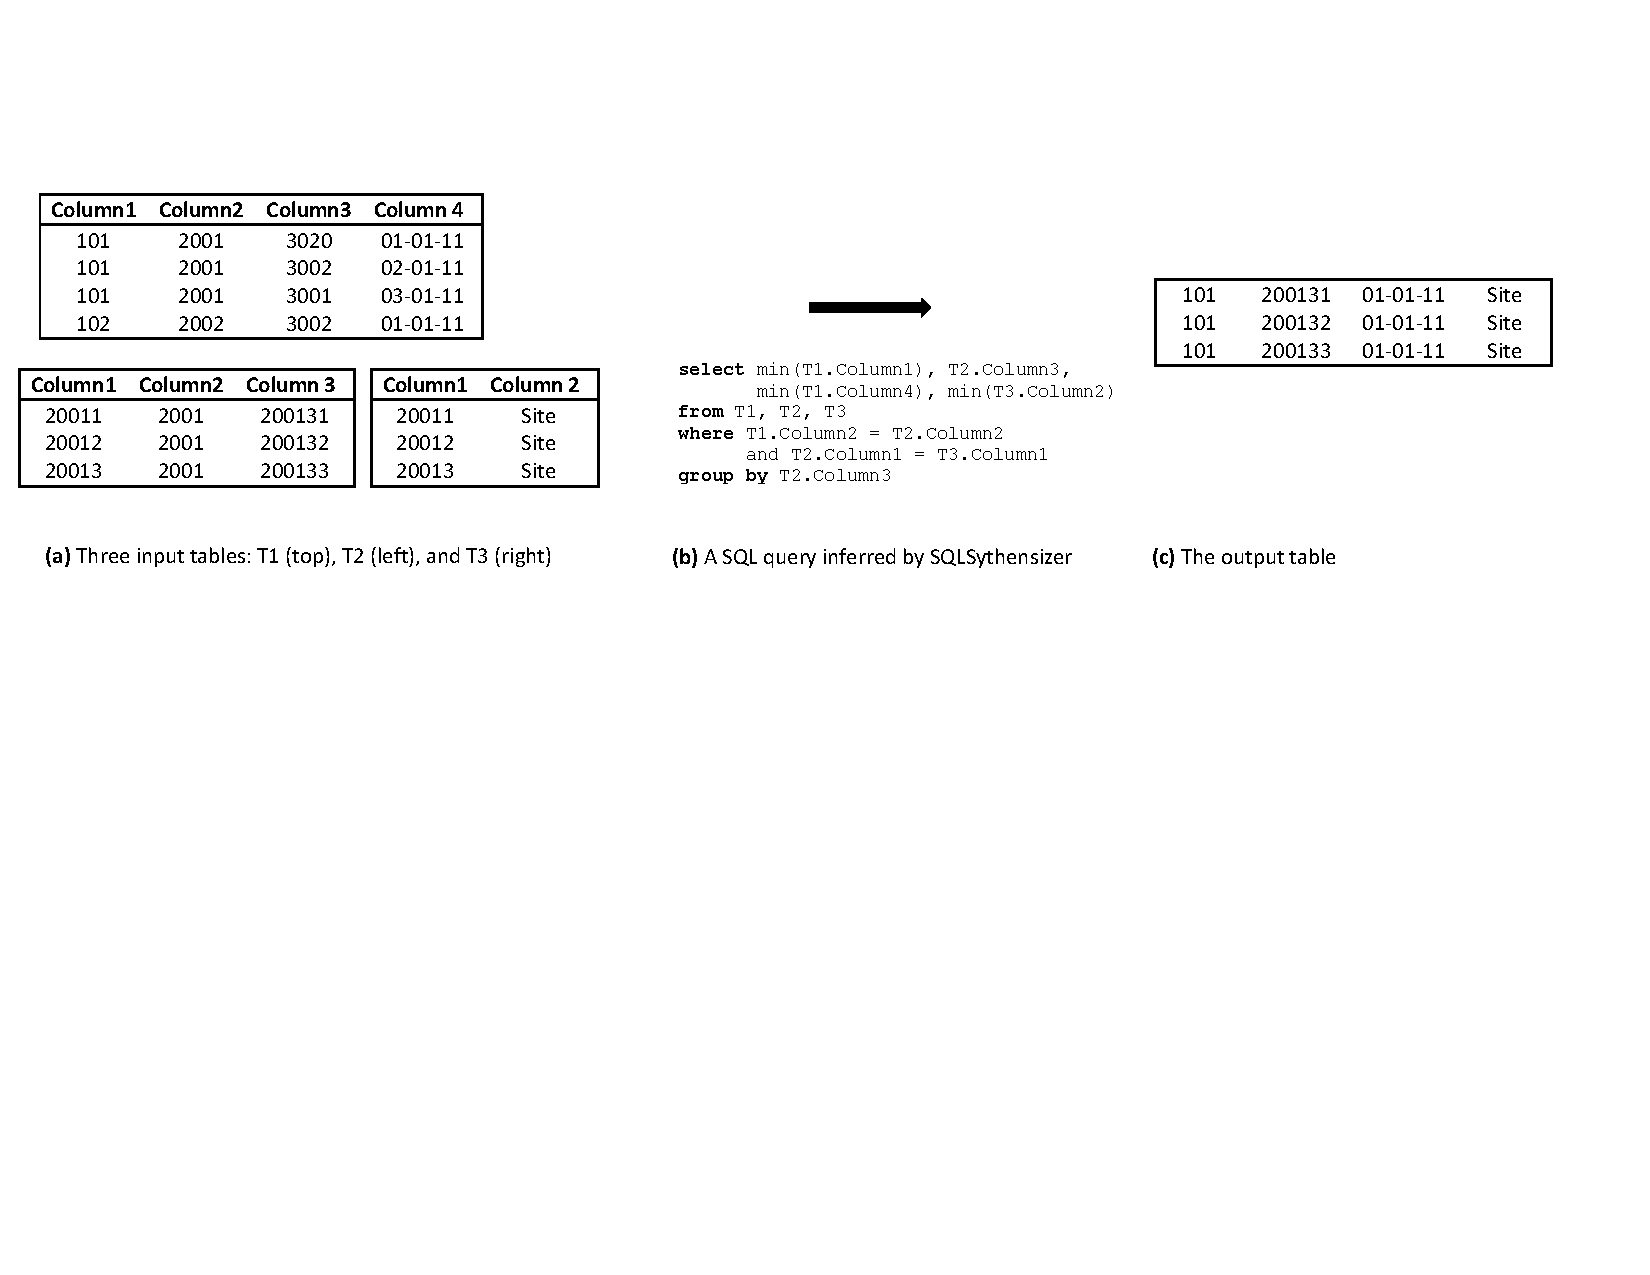
\includegraphics[scale=0.70]{example2}
  \vspace*{-1.0ex}\caption {{\label{fig:example2} Input-output
  examples ((a) and (c)) taken from an online SQL help forum
  thread. \ourtool automatically sythensizes 6 SQL queries that
  can produce the output table from the three input tables.
  (b) shows the highest ranked SQL query.
}}
\end{figure*}

We use a real SQL question from
an online forum\footnote{\url{http://forums.tutorialized.com/sql-basics-113/join-problem-147856.html}} to illustrate
\ourtool's effectiveness.
The question was started by a novice user, who needed help to write a
SQL query to get result from three input tables. In this question, the
novice user described his required query in a few paragraphs of
English, but also include several small, representative input-output
examples as shown in Figure~\ref{fig:example2}, to better express
his intention. 
This question receives no replies as of April 2013 and we speculated that
writing a SQL query to join three tables to produce certain output results
is non-trivial.

We ran \ourtool on the input-output examples
in Figure~\ref{fig:example2}. The tool produced 6 valid answers
in less than 1 minutes, all of which satisfy the given examples. The
highest ranked SQL query is shown in Figure~\ref{fig:example2},
which is quite unintuitive to write. The SQL query in
Figure~\ref{fig:example2}
first joins three input tables
on columns \CodeIn{T1.Column2}, \CodeIn{T2.Column2},
\CodeIn{T2.Column1}, and \CodeIn{T3.Column1} using some
selected columns, and then aggregates the results based on
column \CodeIn{Table2.Column3}'s value. Finally, it
returns the minimal values of columns \CodeIn{T1.Column1}, \CodeIn{T1.Column4}, and \CodeIn{T3.Column2}
from each aggregated group as the results.



